\pl{when we say $O(...)$, we're actually hiding $\log B$ factors; probably should use $\tilde O$?}

\section{Introduction}

The probability that a system outputs for an event should reflect the true frequency of that event: if an automated diagnosis system says 1,000 patients have cancer with probability 0.1, approximately 100 of them should indeed have cancer.
In this case, we say the model is uncertainty calibrated. The importance of this notion of calibration has been emphasized in personalized medicine~\cite{jiang2012calibrating}, meteorological forecasting~\cite{murphy1973vector, murphy1977reliability, degroot1983forecasters,gneiting2005weather, brocker2009decomposition} and natural language processing applications~\cite{nguyen2015posterior, card2018calibration}.
As most modern machine learning models, such as neural networks, do not output calibrated probabilities out of the box~\cite{guo2017calibration, zadrozny2001calibrated, kuleshov2018accurate}, \pl{since you use 'As ...', here should say here that 'researchers } recalibration methods take the output of an uncalibrated model, and transform it into a calibrated probability.
\emph{Scaling} approaches for recalibration---Platt scaling~\cite{platt1999probabilistic}, isotonic regression~\cite{zadrozny2002transforming}, and temperature scaling~\cite{guo2017calibration}---are widely used and require very few samples, but do they actually produce calibrated probabilities?

\emph{We discover that these methods are less calibrated than reported.} Past work approximates a model's calibration error using a finite set of bins. We show that by using more bins, we can uncover a higher calibration error \pldel{for models} on CIFAR-10 and ImageNet.
We show that a fundamental limitation with approaches that output a continuous range of probabilities is that their true calibration error \pl{is actually \emph{unmeasurable}} may never be measurable with a finite number of bins (Example~\ref{ex:continuous-not-calibrated}).

An alternative approach, histogram binning~\cite{zadrozny2001calibrated}, outputs probabilities from a finite set.
Histogram binning can produce a model that is calibrated, and unlike scaling methods we can measure its calibration error, but it is sample inefficient.
In particular, the number of samples required to calibrate scales linearly with the number of distinct probabilities the model can output, $B$~\cite{naeini2014binary}, which can be large particularly in the multiclass setting where $B$ typically scales with the number of classes.
Recalibration sample efficiency is crucial---we often want to recalibrate our models in the presence of domain shift~\cite{hendrycks2019anomaly} or recalibrate a model trained on simulated data, and may have access to only a small labeled dataset from the target domain.

To get the sample efficiency of Platt scaling and the verification guarantees of histogram binning, \emph{we propose \ourcal{}} (Figure~\ref{fig:var_red_binning}).
Like scaling methods, we fit a simple function $g \in \mathcal{G}$ to the recalibration dataset.
We then bin the input space so that an equal number of inputs land in each bin.
In each bin, we output the average of the $g$ values in that bin---these are the gray circles in Figure~\ref{fig:var_red_binning}.
In contrast, histogram binning outputs the average of the label values in each bin (Figure~\ref{fig:hist_binning}).
The motivation behind our method is that the $g$ values in each bin are in a narrower range than the label values, so when we take the average we incur \pl{lower} \pldel{less of an} estimation error.
If $\mathcal{G}$ is well chosen \pl{what does this mean?}, our method requires $O(\frac{1}{\epsilon^2} + B)$ samples to achieve calibration error $\epsilon$ instead of $O(\frac{B}{\epsilon^2})$ samples for histogram binning, where $B$ is the number of model outputs (Theorem~\ref{thm:final-calib}). Note that in prior work, binning the outputs of a function was used for evaluation and without any guarantees, whereas in our case it is used for the method itself, and we show improved sample complexity.

\begin{figure}
     \centering
     \begin{subfigure}[b]{0.32\textwidth}
         \centering
         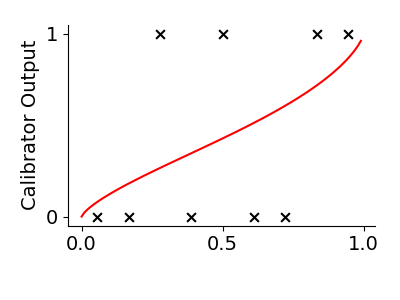
\includegraphics[width=\textwidth]{platt_scaling}
         \caption{Platt scaling}
         \label{fig:platt_scaling}
     \end{subfigure}
     \hfill
     \begin{subfigure}[b]{0.32\textwidth}
         \centering
         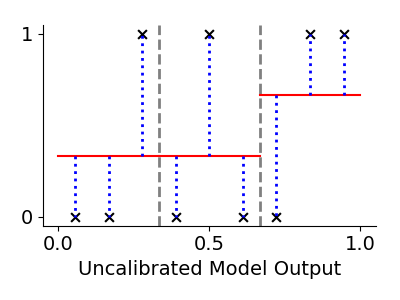
\includegraphics[width=\textwidth]{histogram_binning_with_deltas}
         \caption{Histogram binning}
         \label{fig:hist_binning}
     \end{subfigure}
     \hfill
     \begin{subfigure}[b]{0.32\textwidth}
         \centering
         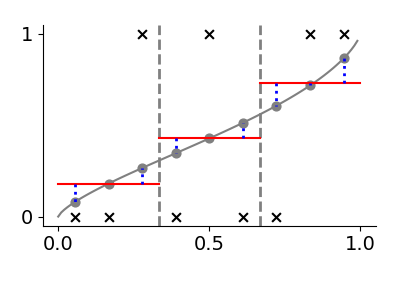
\includegraphics[width=\textwidth]{variance_reduced_binning_with_deltas}
         \caption{\Ourcal{} \pl{remove 'the'}}
         \label{fig:var_red_binning}
     \end{subfigure}
        \caption{
        Visualization of the three recalibration approaches.
        The black crosses are the ground truth labels, and the red lines are the output of the recalibration methods.
        Platt Scaling (Figure~\ref{fig:platt_scaling}) fits a function to the recalibration data, but its calibration error is not measurable.
        Histogram binning (Figure~\ref{fig:hist_binning}) outputs the average label in each bin.
        \Ourcal{} (Figure~\ref{fig:var_red_binning}) fits a function $g \in \mathcal{G}$ to the recalibration data and then \emph{takes the average of the function values (the gray circles)} in each bin.
        The function values have lower variance than the labels, as visualized by the blue dotted lines, which is why our approach has lower variance.
        }
        \label{fig:variance_reduced_illustration}
\end{figure}

Next, we turn to the question of estimating the calibration error. Prior work in machine learning~\cite{nguyen2015posterior, guo2017calibration, hendrycks2019anomaly, kuleshov2015calibrated, hendrycks2019pretraining} directly estimates each term \pl{haven't introduced term, so doesn't make sense; choose another way to explain} in the calibration error from samples (Definition~\ref{dfn:plugin-estimator}). The sample complexity of this plugin estimator scales linearly with $B$. An alternative estimator introduced in the meteorological literature~\cite{brocker2012empirical, ferro2012bias} reduces the bias of the plugin estimator; \emph{we prove that it has sample complexity that scales with $\sqrt{B}$} by leveraging error cancellations across bins.

We run multiclass calibration experiments on CIFAR-10~\cite{krizhevsky2009learningmultiple} and ImageNet~\cite{deng2009imagenet}.
The objective is to minimize the mean-squared error, also known as the Brier score~\cite{brier1950verification}, subject to a calibration error budget~\cite{gneiting2005weather}.
We show that \ourcal{} achieves a better \pl{lower} calibration error than histogram binning, while allowing us to measure the true calibration error.
For example, we get a \emph{35\% lower calibration error on CIFAR-10} and a \emph{5x lower calibration error on ImageNet} than histogram binning if \pl{for} $B = 100$.

% In summary, our contributions are:
% \begin{enumerate}
% \item We show that scaling methods for recalibration are less calibrated than reported.
% \item We introduce the first method, to our knowledge, that has better sample complexity than histogram binning but has a \emph{measurable calibration error}, giving us the best of both worlds of scaling and binning. Our method achieves significantly (up to 5x) lower calibration errors on top-label and per-class calibration on CIFAR-10 and ImageNet.
% \item We show that the method typically used to estimate calibration error is suboptimal, and an alternative estimator from the meteorological community requires fewer samples to measure the calibration error.
% \end{enumerate}

% \tm{Sometimes I do a summary of contribution paragraph for the reviewers to easily see the contribution. doesn't add anything to the quality of the paper, but sometimes useful for paper acceptance .. (As a rushed reviewer sometimes I wanted the authors to have a simple para with a bit more technical term than abstract....)}

% \pl{it's a nice to have if we have space; the use of italics throughout the intro is actually pretty effective}

% \ak{Is this better?}
